\documentclass[11pt]{article}
\usepackage{graphicx,amsmath,amsfonts,amssymb,graphicx} 
\usepackage[varg]{txfonts}
\usepackage{enumerate}
\usepackage{subcaption}
\usepackage{hyperref}
\usepackage{listings}
\usepackage{color}
\urlstyle{tt}

\usepackage{geometry}
\geometry{%
  letterpaper,
  lmargin=2cm,
  rmargin=2cm,
  tmargin=2cm,
  bmargin=2cm,
  footskip=12pt,
  headheight=12pt}
  
\usepackage{lastpage}
\usepackage{fancyhdr}
%\pagestyle{fancy}
%\headheight 35pt

\def\squarebox#1{\hbox to #1{\hfill\vbox to #1{\vfill}}}
\def\qed{\hspace*{\fill}
        \vbox{\hrule\hbox{\vrule\squarebox{.667em}\vrule}\hrule}}
\newenvironment{solution}{\begin{trivlist}\item[]{\bf Solution:}}
                      {\end{trivlist}}
\lstset{
	language=MATLAB,              % choose the language of the code ("language=Verilog" is popular as well)
   tabsize=3,							  % sets the size of the tabs in spaces (1 Tab is replaced with 3 spaces)
	basicstyle=\tiny,               % the size of the fonts that are used for the code
	numbers=left,                   % where to put the line-numbers
	numberstyle=\tiny,              % the size of the fonts that are used for the line-numbers
	stepnumber=2,                   % the step between two line-numbers. If it's 1 each line will be numbered
	numbersep=5pt,                  % how far the line-numbers are from the code
	%backgroundcolor=\color{mygrey}, % choose the background color. You must add \usepackage{color}
	%showspaces=false,              % show spaces adding particular underscores
	%showstringspaces=false,        % underline spaces within strings
	%showtabs=false,                % show tabs within strings adding particular underscores
	frame=single,	                 % adds a frame around the code
	tabsize=3,	                    % sets default tabsize to 2 spaces
	captionpos=b,                   % sets the caption-position to bottom
	breaklines=true,                % sets automatic line breaking
	breakatwhitespace=false,        % sets if automatic breaks should only happen at whitespace
	%escapeinside={\%*}{*)},        % if you want to add a comment within your code
	%commentstyle=\color{BrickRed}   % sets the comment style
}                    
\begin{document}

\title{\bf{CSE397: Assignment \#5}}
\author{Nicholas Malaya \\ Department of Mechanical Engineering \\
Institute for Computational Engineering and Sciences \\ University of
Texas at Austin} \date{} 
\maketitle
\newpage

\subsection*{Problem 1: An inverse problem for Burgers' Equation}

\begin{enumerate}
\item[(1)] Derive a weak form. Use integration-by-parts on the viscous
	   term to derive the weak form of Burgers' equation. 

\begin{solution}
Starting with Burgers' equation in strong form, 
\begin{align}
 u_t + u u_x - \nu u_{xx} = f, 
\end{align}
we multiply by a test function, $p(t,x)$ and integrate over time and space, 
\begin{align}
 \int_0^T \int_0^L (u_t p + u u_x p - \nu u_{xx} p - f p) dx dt = 0. 
\end{align}
Now, we integrate the viscous term by parts, to move a derivative of x
 onto the test function, 
\begin{align}
 \int_0^T \int_0^L (u_t p + u u_x p + \nu u_{x} p_x - f p) dx dt -
 \int_0^T \nu u_x p \bigg|_{x=0}^{x=T} dt = 0. 
\end{align}
Notice that we have introduced a boundary term (and changed the sign of
 the convective operator) by doing this. However,
 $p(0,x)=0$, and therefore this term vanishes. Thus, 
\begin{align}
 \int_0^T \int_0^L (u_t p + u u_x p + \nu u_{x} p_x - f p) dx dt = 0
\end{align}
is our weak form.  
\end{solution}

\item[(2)] Using the Lagrangian functional, derive expressions for the
	   adjoint equation and for the gradient of J with respect to
	   $\nu$. Give weak and strong forms of these equations. 
\begin{solution}

The Largrangian functional is given by: 
\begin{equation}
\mathcal{L} = \int_0^T \int_0^L (u_t p + u u_x p + \nu u_{x} p_x - f p) dx dt
+ \frac{1}{2}\int_{T_1}^T\int_0^L(u-u^{\text{obs}})^2dxdt  
+ \frac{\beta}{2} \int_0^L \nu_x \nu_x dx  
\label{lagrangian}
\end{equation}
Varying this with respect to the test function, $p$, will yield (1) back
 in weak and strong form. Varying with respect to $u$ will return the
 weak form of the adjoint equation which holds for all $\tilde{u}$ which
 obey the same boundary conditions as $u$ (we must integrate $\tilde u_t$
 and $\tilde u_x$ by parts to accomplish this):   
\begin{equation}
\delta_u \mathcal{L} = \int_0^T\int_0^L\left(-\tilde{u} p_t +
					u\tilde{u}_x p + \tilde{u}u_x p  
		 - \nu\tilde{u} p_{xx}\right)dxdt  
+ \int_{T_1}^T\int_0^L(u-u^{\text{obs}})\tilde{u}dxdt = 0.
\end{equation}
As one would expect, this moves backward in time. 


 Now, in order to solve for the strong form, we now need to combine the
 integration from $T_1$ to $T$ with the integral from zero to $T$. In
 order to do this, we multiply the second integral by a function that is
 zero below $T_1$, and 1 past it. This is actually the ``Heavyside
 function''. The resulting equation is then, 
\begin{equation}
\delta_u \mathcal{L} = \int_0^T\int_0^L \left( -\tilde{u} p_t -
					\tilde{u}(u p)_x + \tilde{u}u_x p  
		 - \nu\tilde{u} p_{xx}
+ H(t-T_1)(u-u^{\text{obs}})\tilde{u} \right)dxdt = 0.
\end{equation}
Now, we move $\tilde u$ out of the parenthesis, 
\begin{equation}
\delta_u \mathcal{L} = \int_0^T\int_0^L \tilde u \left( - p_t -
					(u p)_x + u_x p  
		 - \nu p_{xx}
+ H(t-T_1)(u-u^{\text{obs}}) \right) dxdt = 0.
\end{equation}
Remember that $\tilde u$ is arbitrary. Everything in the parenthesis above must
 therefore be equal to zero, and our strong form is:
\begin{equation}
- p_t - (u p)_x + u_x p - \nu p_{xx} + H(t-T_1)(u-u^{\text{obs}}) = 0.
\end{equation}

\end{solution}
\end{enumerate}

Finally, the variation with respect to $\nu$ is, 
\begin{equation}
 \delta_\nu \mathcal{L} = \frac{\beta}{2} \int^L_0 \nu_x \tilde \nu_x dx +
  \int_0^T \int_0^L \tilde \nu u_x p_x dx dt. 
\end{equation}
This is the weak form of the gradient. In order to arrive at the strong
form, we perform the simple judo kata of moving the differential
operator from $\tilde v_x$, 
\begin{equation}
  \int_0^T \int_0^L \tilde \nu u_x p_x dx dt -\frac{\beta}{2} \int^L_0
   \nu_{xx} \tilde \nu dx.
\end{equation}
Next, move $\beta$ into the integral, and pull out the time integration, 
\begin{equation}
 \int_0^T \left[ 
	   \int_0^L \tilde \nu u_x p_x dx -\frac{\beta}{2} \int^L_0
	   \nu_{xx} \tilde \nu dx 
       \right] dt
\end{equation}
finally, combine the spatial integration operators, 
\begin{equation}
 \int_0^T \left[ 
	   \int_0^L \tilde \nu \left(u_x p_x - \frac{\beta}{2} \nu_{xx}
			       \right) dx \right] dt.
\end{equation}
Now, we have isolated $\tilde \nu$, which can be arbitrary. Thus, the
terms in the parenthesis must be equal to zero, and the strong form
appears as: 
\begin{equation}
 u_x p_x - \frac{\beta}{2} \nu_{xx} = 0.
\end{equation}
%
%
%
%
%
%

\newpage
\subsection*{Problem 2}
\textbf{Inverse elliptic parameter estimation, continued from assignment
4.} We solve 
the inverse problem for the advection-diffusion equation on $\Omega =
[0, 1] \times [0, 1]$: 
\begin{equation}
\min_a J(m) = \frac{1}{2}\int_\Omega(u-u^{\text{obs}})^2dx +
 \frac{\beta}{2}\int_\Omega (\nabla m \cdot \nabla m)dx \tag{8}
 \label{2cost} 
\end{equation}
where $u$ is the solution of
\begin{align}
-\nabla\cdot(m\nabla u) + v\cdot\nabla u &= f \text{ in } \Omega
 \\ 
u &= 0 \text{ on } \partial \Omega 
\end{align}
with the advective velocity $v = (v_1 , v_2 )$, regularization parameter
$\beta > 0$ and measurement data $u^{\text{obs}}$ , which are obtained by
solving the state equation with $m(x, y) = 2$ for $(x - 0.5)^2 + (y -
0.5)^2 \le 0.04$ and $m(x, y) = 8$ otherwise (and adding noise). 
\begin{enumerate}
\item[(a)]Find an optimal regularization parameter $\beta$ found from the
	  discrepancy criterion.

\begin{solution}
The discrepancy criterion is defined as $(u-u^{\text{obs}}) \approx
 \delta$. We find $\delta = 0.02$ by adding the following lines to the
 solution file: 
 \begin{lstlisting}
  if(noise==0)
    noise = datanoise * max(abs(X(UDI))) * randn(length(UDI),1);
    delta = norm(noise)
  end
 \end{lstlisting}
 Where we also add this ``noise'' variable to the data. We now calculate
 the difference between $\delta$ and $(u-u^{\text{obs}})$ using, 
 \begin{lstlisting}
  err=norm(X(UDI) - X(UI))-delta
 \end{lstlisting}
We now iterate over choices of regularization, to find an optimal
 $\beta$. The curve is relatively flat, indicating that the inverse
 problem is not particularily sensitive to choice of regularization
 parameter, but the optimal value appears to be right around $\beta
 \approx 1e-10$. (e.g I found the ``err'' above was only .001 for $\beta
 = 0.001$, which indicates it does not change greatly for several orders
 of magnitude.)
 
\end{solution}


\item[(b)]Extend the COMSOL implementation elliptic\_GN\_ip of the
	  Gauss-Newton method using the advection velocity
	  $v=(30,0)$. Report the number of Gauss-Newton and of overall
	  CG iterations for a discretization of the domain with $10
	  \times 10$, $20 \times 20$, $40 \times 40$ and $80 \times 80$
	  linear finite elements and give the number of unknowns used to
	  discretize the coefficient function $m$ (which is called a in
	  the implementation) for each of these meshes. Discuss how the
	  number of iterations changes as more parameters are used. 

\begin{solution}
To introduce $v=(30,0)$ into the code, we added the following lines:
\begin{lstlisting}
fem.equ.expr.v1 = '30';
fem.equ.expr.v2 = '0';

% weak forms to make up data ud, state, adjoint and control equation
fem.equ.expr.goal    = '-(atrue*(udx*udx_test+udy*udy_test)
+v1*udx*ud_test+v2*udy*ud_test-f*ud_test)';
fem.equ.expr.state   = '-(a*(ux*ux_test+uy*uy_test)
+v1*ux*u_test+v2*uy*u_test-f*u_test )';

fem.equ.expr.incstate   = ['-(a*(delta_ux*delta_px_test+delta_uy*' ...
   'delta_py_test)+v1*delta_ux*delta_p_test+v2*delta_uy*delta_p_test
+delta_a*(ux*delta_px_test+uy*delta_py_test))'];
fem.equ.expr.incadjoint = ['-(a*(delta_px*delta_ux_test+delta_py*' ...
   'delta_uy_test)+v1*delta_ux_test*delta_p+v2*delta_uy_test*delta_p
+delta_u*delta_u_test )'];
fem.equ.expr.inccontrol = ['-(gamma*(delta_ax*delta_ax_test+delta_ay' ...
   '*delta_ay_test)+(delta_px*ux+delta_py*uy)*delta_a_test)'];
\end{lstlisting}
We also need to adjust the values in
\begin{lstlisting}
fem.mesh = meshmap(fem, 'Edgelem', {1,20,2,20});
\end{lstlisting}
so for a $10\times 10$ grid I would set $10$ instead of $20$, and so on 
 for 20,40, 80, etc. 
 
\begin{center}
\begin{tabular}{l||l|l}
 Mesh & Gauss-Newton Iterations & Overall CG iterations\\
\hline\hline
$10\times 10$ & 7 & 41\\
$20\times 20$ & 6 & 29\\
$40\times 40$ & 7 & 42\\
$80\times 80$ & 7 & 49
\end{tabular}
\end{center}

Aside from the $20\times20$ mesh, the number of Newton iterations
 remains very nearly the same! The CG iterations also remain the same or only
 increase slightly with the mesh-size. This is a remarkable result,
 because it implies the Newton iterations are independent of problem
 size. 

\end{solution}

\item[(c)]To avoid over-solving of the CG system in early Newton steps,
	  where we are still far away from the solution and thus cannot
	  benefit from the fast local convergence properties of Newton's
	  method, the implementation uses the stopping
	  criterion. Discuss the behavior.  


\begin{solution}
In order to account the differenct stopping criteria, I added the following lines:
\begin{lstlisting}
    stopping = 0.5;
    stopping = min(0.5, sqrt(gradnorm/gradnorm_ini));
    stopping = min(0.5, gradnorm/gradnorm_ini);
\end{lstlisting}
where we comment out all but the criterion we wish to use. Also, we are 
 going back to a mesh of $20\times 20$ elements (the $80\times 80$ is
 exceedingly slow on the node provided). 

\begin{center}
 \begin{tabular}{l||l|l}
  Method & Gauss-Newton Iterations & Overall CG iterations\\
  \hline\hline
  $\eta_k=0.5$ & 12 & 47\\
  $\eta_k=\min(0.5,\sqrt{\|g_k\|/\|g_0\|})$ & 7 & 50\\
  $\eta_k=\min(0.5,\|g_k\|/\|g_0\|)$ & 6 & 64
 \end{tabular}
\end{center}

In summary, we see exactly the behavior as predicted in assignment
 two. For the choice $\eta_k=0.5$ we see a linear convergence behavior
 which is the  reason why we needed the most Gauss-Newton iterations in
 this case. In  the second case, as soon as we get close to the minimum
 (the point  where the gradient is zero), we are getting a convergence somewhere
 in between  linear and quadratic convergence. 
 For the final choice, we are getting quadratic convergence as soon as we get close to
 the point where the gradient is zero. 

 However, the total number of CG iterations needed in
 order is increased for each subsequent scheme. 
 For the first choice we needed the least number of CG iterations. 

 What we see here is that if we want to see the superlinear or quadratic
 convergence in the second or third choices, we require more CG
 iterations. Ultimately, the decision on which stopping criterion to use depends on
 balancing the desire to minimize CG iterations per newton solve against
 taking advantage of the superior convergence properties of the later
 criterion. 

\end{solution}

\item[(d)]The ill-posedness of inverse problems is closely related to
	  the spectrum (i.e., the eigenvalues) of the involved
	  operators. Compute the eigenvalues of the reduced Hessian at
	  the solution of the problem for a mesh with $20 \times 20$
	  elements. Since the Hessian is not explicitly available and
	  can only be applied to vectors, there are 2 possibilities to
	  access its eigenvalues: 
\begin{enumerate}
\item[$\bullet$] Build the Hessian matrix explicitly by applying it to
	     unit vectors and compute the eigenvalues of the resulting
	     matrix. 
\item[$\bullet$] There exist iterative methods for computing
	     eigenvalues of a matrix that require only the application
	     of the matrix to vectors. Compute the largest
	     100 eigenvalues using an iterative method. 
\end{enumerate}
Plot the spectrum of the reduced Hessian with and without regularization 
	  and discuss the result. 

\begin{solution}
I added the following lines, to calculate the first 100 eigenvalues using
 the second (recommended) method: 
\begin{lstlisting}
eigsolve = @(V)elliptic_apply(V,chi,W,A,C,R,X);
lambda = eigs(eigsolve, size(C,2),100,'lm');
figure;
plot(lambda);
\end{lstlisting}
The spectrum of the Hessian is plotted below, for cases using regularization,
 and not. 
 \begin{figure}[!htb]
  \centering
  \begin{subfigure}[bh]{0.45\textwidth}
   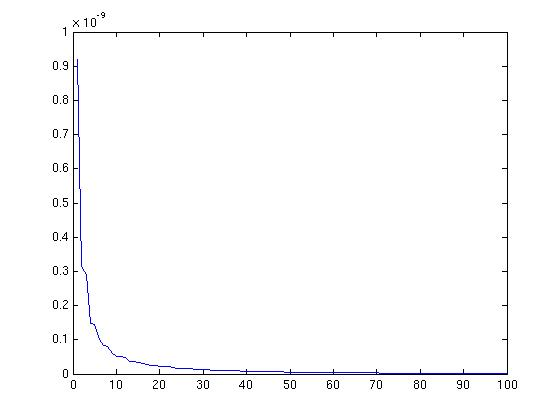
\includegraphics[width=\textwidth]{figs/noreg.jpg}
  \end{subfigure}%
  \begin{subfigure}[bh]{0.45\textwidth}
   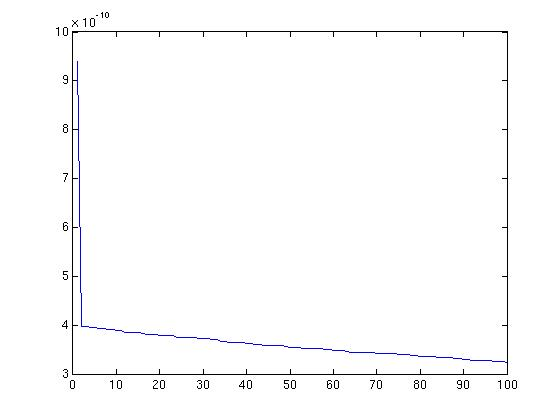
\includegraphics[width=\textwidth]{figs/regularization.jpg}
  \end{subfigure}
  \caption{The unregularized (left) and regularized (right) spectrum of
  the Hessian. }
 \end{figure}

As one can see, the larger eigenvalues are nearly the same. However,
 without regularization the eigenvalues converge to zero rapidly, which
 results in what is, due to numerical error, essentially a non-positive
 definite matrix. In other words, the regularization accomplishes
 precisely what we desired: it prevents the small eigenvalues from
 converging to zero while keeping the large eigenvalues close to the
 unregularized values. 

\emph{Note: did we cover the Lanczos method in class? I don't think I am
 familiar with this technique, but it is interesting. }

\end{solution}


%\item[(e)]\textit{Optional:}Replace the Tikhonov regularization by total
%	  variation regularization and report the results for different
%	  meshes. 
\end{enumerate}

%\newpage
%\subsection*{Code}
%Here is the code for part c:
%\lstinputlisting{code/elliptic_sd_ip_adv_TV.m}
\end{document}